\documentclass[letterpaper,10pt]{article}

\usepackage{titling}
\usepackage{listings}
\usepackage{url}
\usepackage{setspace}
\usepackage{subfig}
\usepackage{sectsty}
\usepackage{pdfpages}
\usepackage{colortbl}
\usepackage{multirow}
\usepackage{multicol}
\usepackage{relsize}
\usepackage{amsmath}
\usepackage{wasysym}
\usepackage{fancyvrb}
\usepackage{amssymb}
\usepackage{ifsym}
\usepackage{amsmath,amssymb,amsthm,graphicx,xspace}
\usepackage[titlenotnumbered,noend,noline]{algorithm2e}
\usepackage[compact]{titlesec}
\usepackage{XCharter}
\usepackage[T1]{fontenc}
\usepackage{tikz}
\usetikzlibrary{arrows,automata,shapes,trees,matrix,chains,scopes,positioning,calc}
\tikzstyle{block} = [rectangle, draw, fill=blue!20, 
    text width=2.5em, text centered, rounded corners, minimum height=2em]
\tikzstyle{bw} = [rectangle, draw, fill=blue!20, 
    text width=4em, text centered, rounded corners, minimum height=2em]

\definecolor{namerow}{cmyk}{.40,.40,.40,.40}
\definecolor{namecol}{cmyk}{.40,.40,.40,.40}

\let\LaTeXtitle\title
\renewcommand{\title}[1]{\LaTeXtitle{\textsf{#1}}}


\newcommand{\handout}[5]{
  \noindent
  \begin{center}
  \framebox{
    \vbox{
      \hbox to 5.78in { {\bf ECE356: Database Systems } \hfill #2 }
      \vspace{4mm}
      \hbox to 5.78in { {\Large \hfill #4  \hfill} }
      \vspace{2mm}
      \hbox to 5.78in { {\em #3 \hfill} }
    }
  }
  \end{center}
  \vspace*{4mm}
}

\newcommand{\lecture}[3]{\handout{#1}{#2}{#3}{Lecture #1}}
\newcommand{\tuple}[1]{\ensuremath{\left\langle #1 \right\rangle}\xspace}

\addtolength{\oddsidemargin}{-1.000in}
\addtolength{\evensidemargin}{-0.500in}
\addtolength{\textwidth}{2.0in}
\addtolength{\topmargin}{-1.000in}
\addtolength{\textheight}{1.75in}
\addtolength{\parskip}{\baselineskip}
\setlength{\parindent}{0in}
\renewcommand{\baselinestretch}{1.5}
\newcommand{\term}{Winter 2018}

\singlespace


\begin{document}

\lecture{ 34 --- Recovery: Repairing Inconsistent Data }{\term}{Jeff Zarnett}

\section*{Inconsistent data? In my database? It's more likely than you think!}

Inconsistent databases are a difficult problem for database designers to deal with. As the definition of inconsistent suggests, one or more integrity constraints have been violated, and one might conclude that queries on the database would be impossible or the answers meaningless. Research on the subject, specifically in the fields of repairing inconsistencies and answering queries despite the status of the database, has provided several options. The works we examine restrict themselves to relational databases, and not any of the other possible types.

We cannot proceed without first providing a working definition of what is meant when we say that a database is consistent. We say a database $D$ is \textit{consistent} if $D$ satisfies the set of integrity constraints $C$ in the standard sense \cite{CQI}. If any of these constraints are not met, the database is \textit{inconsistent} (or has inconsistencies). When there are inconsistencies whereby there are multiple tuples reflecting the same real-world entity, we name that a \textit{cluster}~\cite{CA}.

The obvious source of how databases may become inconsistent is: errors. Data can be entered that violates integrity constraints. That can happen if the database was implemented without certain important integrity constraints (e.g., foreign keys) added, or a new rule is being added. It can also happen because database integrity constraints can be turned off (yikes!) which is usually intended for mass data import, or perhaps because the database engine (myISAM anyone?) just does not enforce those constraints. So in all cases, the inconsistency was added in error. 

However, it is not the case, that by simply relying on error-detection and rule enforcement, we can be certain that no inconsistencies will ever arise. We will look at some ideas of how databases may become inconsistent in the first place, aside from the obvious answer of errors. Papers \cite{CQI} and \cite{CQ} offer some plausible scenarios where inconsistencies may be introduced. The first is from data warehousing; when data is imported from various sources and may need cleaning before storing. The second is database integration; when some data is stored across many databases stitched together, there may be different constraints at a local level than at the higher level, resulting in a locally consistent, yet globally inconsistent, database. It is possible that integrity checking may simply be too costly from a performance standpoint, and the database must proceed without it. Finally, we might, under some circumstances, choose to allow a temporary inconsistency, such as warehouse stock levels being allowed to fall below a minimum when replenishments have already been ordered. It is clear from these three scenarios that there exist plausible reasons why a database might be inconsistent, and why this subject is not rendered irrelevant in an error-free system.

We would like the answer from a query against an inconsistent database to be the same as that of the consistent database, but with partial information, we may not know what the consistent database would return. At the very least, we are interested in getting a consistent answer to a query, even in the presence of inconsistent data. We may also be interested in repairing the database, so that the inconsistencies may be removed entirely.

\subsection*{Repairing Inconsistencies}
When presented with an inconsistent database, we might be able to repair it. The nature of the repair will obviously be context-dependent. The basic definition of a repair $D'$ of a database $D$ is that $D'$ is a modification of $D$ such that $D'$ meets the constraint set $C$.

\paragraph{Basic Principles of Repairs}
There are infinitely many such database repairs that can be performed. We add a further restriction; that the new database $D'$ is changed only minimally from the original $D$. Making the minimal set of changes necessary to meet all constraints $C$ has nice properties: if a database is consistent, then the minimal repair is to do nothing ($D'$ is equal to $D$). Furthermore, we will always be able to find a repair to the the database, since we can make changes as needed to reach a consistent state, although in the worst case, it may mean emptying the database entirely. \cite{CQI}

With that in mind, it is sometimes undesirable to make the minimal set of changes, because that may simply be deletion of the offending tuple(s). While deletion may bring the database into a consistent state, it also may mean data loss, and that is generally not our first choice. We are therefore forced to keep our minds open to repairs that are not the minimal set of changes, but as minimal as possible without data loss.

We will now look at an example using table of employee salaries, Table~\ref{inconsistent1}. In this example, we show only a subset of this relation; columns ``employee\_name" and ``salary" are depicted. The sole constraint is that each employee may have only one salary.

\begin{table}[h]\begin{center}
        \begin{tabular}{r | c  c} 
					salaries & employee\_name & salary \\ \hline
	           		 & J. Page  & 50 000 \\ 
	         		 & J. Page  & 80 000 \\ 
					 & V. Smith & 35 000 \\ 
					 & M. Stowe & 75 000 \\ 
        \end{tabular}
        \caption[Inconsistent Salaries Table]{Inconsistent Salaries Table~\cite{CQ}\label{inconsistent1}}
\end{center}\end{table}

The constraint is violated for the user ``J. Page"; he has two salaries (rows 1 and 2 in Table~\ref{inconsistent1}) - \$50~000 and \$80~000 (cluster size of 2). There are two possible repairs that we can make to this database, depicted in Table~\ref{consistent1} and Table~\ref{consistent2}:

\begin{table}[h]\begin{center}
        \begin{tabular}{r | c  c} 
					salaries & employee\_name & salary \\ \hline
	         		 & J. Page  & 80 000 \\ 
					 & V. Smith & 35 000 \\ 
					 & M. Stowe & 75 000 \\ 
        \end{tabular}
        \caption[Possible Repair of Salaries Table (Option 1)]{Possible Repair of Salaries Table (Option 1) \cite{CQ}\label{consistent1}}
\end{center}\end{table}

\begin{table}[h]\begin{center}
        \begin{tabular}{r | c  c} 
					salaries & employee\_name & salary \\ \hline
	           		 & J. Page  & 50 000 \\ 
					 & V. Smith & 35 000 \\ 
					 & M. Stowe & 75 000 \\ 
        \end{tabular}
        \caption[Possible Repair of Salaries Table (Option 2)]{Possible Repair of Salaries Table (Option 2) \cite{CQ}\label{consistent2}}
\end{center}\end{table}

Rows 3 and 4 of Table~\ref{inconsistent1} are unchanged (as this is a minimal repair), and the two options are to delete either the first row (Table~\ref{consistent1}) or the second (Table~\ref{consistent2}). In either case, we return to a consistent database, because the sole constraint is now correctly enforced. Bertossi and Chomicki clearly demonstrate in~\cite{CQ} an important point: throwing away all tuples that participate in the violation results in the loss of J. Page's data. They overlook the minor point that doing so would not be the minimal set of changes to the system - throwing away one would be enough.

There are some specific circumstances under which we might face infinitely many or infeasibly many repairs; such as how to repair a string such that it is unique in the relation. The number of possible strings which meet this condition is infinite (though it may be constrained from infinite to infeasible by limiting the string length attribute (for example, to 255 characters). Under those circumstances, the repair we undertake is to insert a \texttt{null} into that attribute, and therefore compress the infinite or infeasible set down to one possible repair \cite{CQ}. The proponents of this system acknowledge that it is imperfect, however, because the relational data model may forbid a null in that attribute.

\paragraph{Specifying Repairs with Annotations}
The pressing question now is what repairs to perform. Annotated logic, specifically, \textit{Annotated Predicate Calculus} as in \cite{CQ}, provides a method. We must move beyond classical logic, otherwise inconsistencies (logical contradictions) would prove problematic. In APC, we annotate database atoms (components) with true ($t$), false ($f$), contradictory ($\top$), and unknown ($\bot$). Below in Figure \ref{TruthLattice} is the lattice of logical values. In this figure, the intersection points represent truth values ($t$, $f$, et cetera) and the edges represent paths along which reasoning moves when additional data is found.

The truth values in the lattice are as follows, all from \cite{CQ}:

\begin{itemize}
\item \textit{Basic Values}: $t$, $f$, $\top$, and $\bot$, as explained in the preceding paragraph. 
\item \textit{Database Values:} $t_d$ for atoms in the original database and $f_d$ for those not in it.
\item \textit{Constraint Values:} $t_c$ and $f_c$ to annotate database literals appearing in the disjunctive normal form of the constraints. Built-in atoms in the constraints receive simply $t$ and $f$.
\item \textit{Advisory Values:} $t_a$ and $f_a$ are used to resolve situations where the database does not conform to the integrity constraints. 
\end{itemize}

\begin{figure}[!h]
  \centering 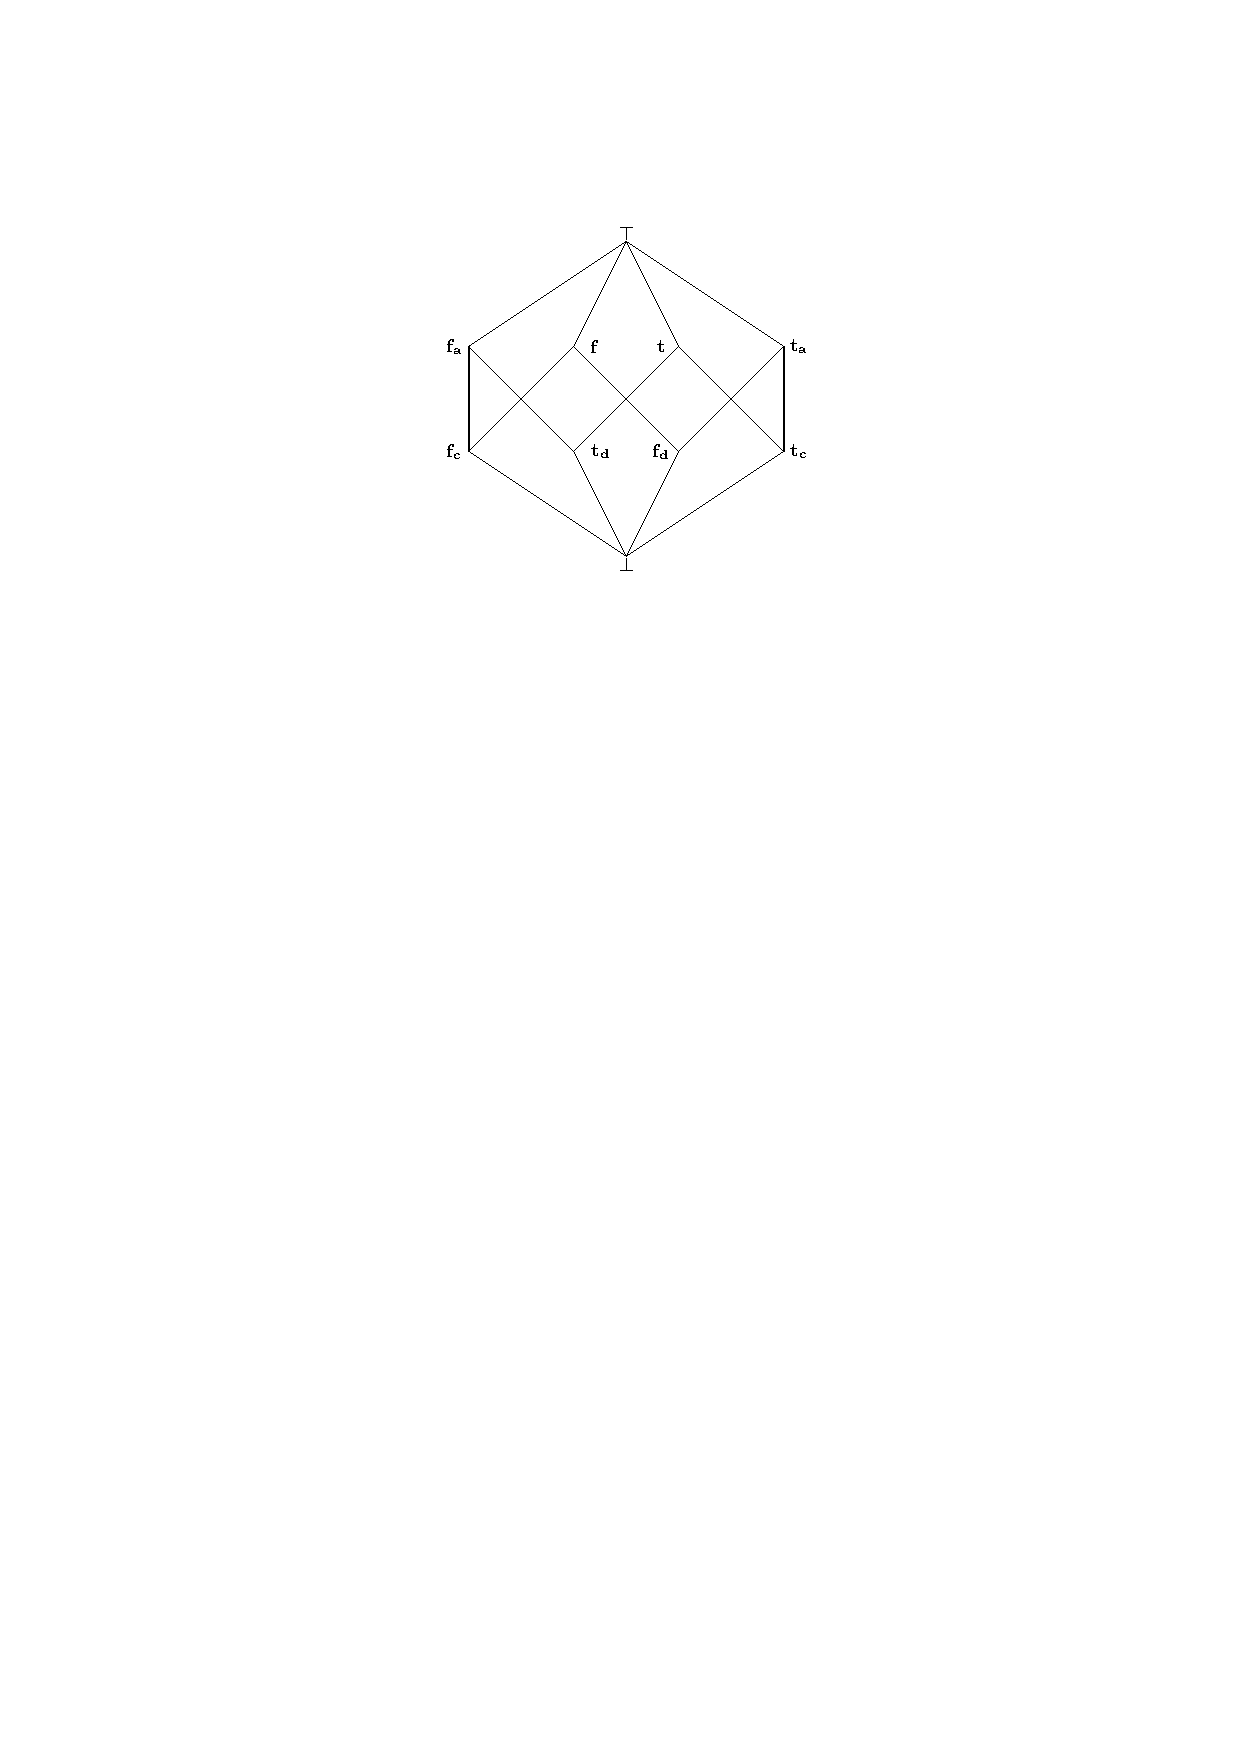
\includegraphics[width=3.5in]{images/TruthLattice.pdf}
  \caption[Truth Value Lattice]{Truth Value Lattice \cite{CQ}}
  \label{TruthLattice}
\end{figure}


Using Figure \ref{TruthLattice}, we provide some clarifying examples. In the simplest case, if we have something true in the database ($t_d$), and true in the constraints ($t_c$), then we can move simply to true ($t$), without problem. If we find something true in the database ($t_d$) yet false according to the constraints ($f_c$), then we can move to $f_a$ - suspected false. If we have an irresolvable conflict, for example, finding one thing certainly true and the other certainly false, we move to $\top$ (showing there is nothing we can do to resolve this).

We consider data to be fallible, but constraints to be correct. Thus, if an atom gets both $t_d$ and $f_c$ (true in the database but not permitted by the constraints), we will resolve that conflict as $f_a$; we think it should be false. At the end of the evaluation, in order to repair the database, things we believe to be false will be removed, and things we believe to be true will be inserted into the database. Bertossi and Chomicki in \cite{CQ} assert that for every repair to a database $D$ with respect to constraints $C$, there is a one-to-one relationship with a model of a minimal set of atoms tagged $f_a$ and $t_a$.

If we apply this principle to an inconsistent database, then the results we will get will indicate our best course of action. The results received will simply be a set of advice: add this; delete that. A program can use the set of advisory values to repair the database.

\paragraph{Specifying Repairs with Logic Programs}

A reference in \cite{CQ} presents a way to create a disjunctive program out of the set of advisory clauses produced using the annotated logic method. This program is used to process that advice and produce a repaired database. However, the program uses the annotations as additional data points, and it is therefore not an annotated (i.e. standard) logic program. Such a program will work for arbitrary first-order queries and for arbitrary constraints.


We can also make use of a logic program alone to find repairs. In \cite{CQ} we consider a logic program with exceptions to these rules. The exceptions naturally have a higher priority than the rules. Most of the time, when we repair a database, most data is preserved, but some tuples will be removed. We can combine the appropriate logic program with the idea of logical consequence, and use this to compute repairs. To do so, we must find atoms true in every answer set of the program. This approach functions for all first-order queries, but it may be impractical because the size can quickly get out of hand.

\paragraph{Aggregate Queries}

Aggregate queries are important to databases. Basic operators like \texttt{MIN}, \texttt{MAX}, and \texttt{SUM} are valid queries and should not be excluded. It might be possible that some such queries could be expressed as a first order query, but in \cite{CQ} it is acknowledged that we cannot handle such things using query transformation. 

In some circumstances, the answers to aggregate queries are easy. If we look once again at the examples in Tables \ref{inconsistent1}, \ref{consistent1}, and \ref{consistent2}. As an example, we want to select the minimum salary. V. Smith's salary of \$35~000 is returned under all possible repairs. If instead we sought the maximum, both repairs offer different answers. The solution Bertossi and Chomicki present is that we cannot return a single answer. Instead, we return an interval where the minimum is the lower bound from all possible repairs, and the maximum is the upper bound. In this example, we consider [75~000,~80~000] to be a consistent answer to the aggregation query \cite{CQ}. 



\paragraph{Open Issues}

The major open issue they identify is how to deal with global constraints in a composite database system. It is unclear what a consistent answer is in such a context, and similarly unclear what a repair means \cite{CQ}. Bertossi and Chomicki further suggest that they are uncertain about how we can query such a composite system.

The final suggestion they put forward is to move this mechanism into the database management system. This would allow soft integrity constraints (not explicitly enforced), and different users could have different constraints, should they so choose. Under these circumstances, different consistent answers are returned depending on the query's origin.

\subsection*{Query Transformation}

Bertossi and Chomicki presented another option: query transformation. Instead of modifying the database and then running the query on the new database, we transform the query and run it against the unaltered database. We change the query such that for every possible database $D'$ the answers to said query is equal to the consistent answers (in light of constraints $C$ in the original database $D$).

As in \cite{CQ}, we will consider first-order queries, and only universal integrity constraints. We iterate the transformation of the query by conjoining the \textit{residues} to the results of the query, until the query in iteration $n$ is identical to that in $(n-1)$ \cite{CQ}. If there are no residues, then the query needs no alterations.

\paragraph{Residues}
But what is a residue? Consider the following example constraint set from \cite{CQ}:
\begin{center}
$C = \{\forall x.[R(x) \bigvee \neg P(x) \bigvee \neg Q(x)], \forall x.[P(x) \bigvee \neg Q(x)] \}$ 
\end{center}

We will focus on $Q(x)$ as our target query. The residue of $Q(x)$ with respect to the first constraint is $R(x) \bigvee \neg P(x)$; if the constraint and $Q(x)$ are true, then the residue must also be. The residue with respect to the second constraint is $P(x)$. Finally, the $\neg Q(x)$ component does not have any residues, because the integrity constraints do not constrain it. It is not necessary in this example, but in general, we might need to iterate the procedure, because the residues might themselves have residues.

Instead of running the query $Q(x)$, we ask $Q(x)$ together with each of its residues. More formally, it is $Q(x)$ is logically AND-ed with each residue, as follows:

\begin{center}
$Q(x) \bigwedge (R(x) \bigvee \neg P(x)) \bigwedge P(x)$
\end{center}

The effect of this altered query is to return only the answers to $Q(x)$ for which the constraints hold. Looking at the previous example of Table~\ref{inconsistent1}, the modified query will ask for the names and salaries of all employees ($Q(x)$) where there is only one entry in the relation for that user (the residue, derived from the uniqueness constraint). This will return two tuples (V. Smith and M. Stowe). No data will be returned for tuples where there is a violation (J. Page), so no data is shown reflecting our uncertainty about his salary.

\paragraph{Algorithmic Validity} Arenas, Bertossi, and Chomicki acknowledge that the algorithm hangs on three fundamental principle: soundness, completeness, and termination. While these are not examined in \cite{CQ}, they reference \cite{CQI}, and all three principles are examined therein.

The soundness principle is the most obvious - every answer to the altered query must be a consistent answer to the original. The soundness principle is shown for all universal or non-universal but domain-independent queries. However, this excludes non-universal yet domain dependent queries like $\exists x \neg P(x)$ \cite{CQI}.

Completeness is necessary so that every consistent answer to the original query appears as an answer to the transformed one. They prove completeness for binary and generic constraints, but do not prove it in general. In fact, in the event of disjunctive or existential queries, this method may fail to produce all answers \cite{CQ}. 

Finally, termination means that there will always be a reachable point at which we may stop the query modification iterations because the query no longer changes between iterations. Fortunately, as long as the constraints set is acyclic, then termination occurs for any kind of  query~\cite{CQI}\cite{CQ}.

\paragraph{Open Issues}
If we apply query transformation to the initial database in Table~\ref{inconsistent1}, this will certainly return only the consistent answers from the database (V. Smith and M. Stowe). Neither of the tuples for J.Page will be returned, because they are inconsistent. This may sometimes be desirable, if we do not wish to report information we are uncertain about. However, under some circumstances, it is probably undesirable to simply ignore the tuples that are inconsistent. Surely J. Page would prefer that the discrepancy in his paycheque be alerted to someone rather than have his information not shown in the accounting department's reports. To that end, he would almost certainly prefer to take home the lower amount than nothing at all. Query rewriting is useful, but not a complete solution.

The analysis in \cite{CQI} shows that query rewriting fails in the case of a disjunctive or existential queries, but only fails in the completeness category. The methodology is intended only to handle universal integrity constrains, and therefore existential qualifiers present problems. Arenas, Bertossi, and Chomicki assert that existential qualifiers may lead to co-NP-completeness, and computational feasibility issues prevent the fulfillment of the completeness criterion. 


\bibliographystyle{alphaurl}
\bibliography{356}


\end{document}
